\documentclass[12pt,a4paper,spanish]{book} 
\usepackage{babel}
\usepackage [T1]{fontenc}
\usepackage [latin1]{inputenc}
\usepackage{graphicx}
\usepackage{array}
	  \oddsidemargin 0in
      \textwidth 6.75in
      \topmargin 0in
      \textheight 10.0in
      \parindent 0em
      \parskip 2ex
\usepackage{anysize}
\marginsize{3cm}{2cm}{1.0cm}{1.0cm}

\pagestyle{plain}

\begin{document} 
\title{
\begin{table}[!h]
	\begin{tabular}{m{2cm}m{15cm}}
		\multicolumn{1}{l}{}
		 
\includegraphics[scale=0.25, bb=0 0 0 0]{images/logo-fiuba.png} & 
		 \begin{center}
		 	\begin{LARGE}
				Universidad de Buenos Aires	\linebreak \linebreak		 							Facultad de Ingenier\'{i}a  \linebreak \linebreak
				7112 - Estrucutra de las Organizaciones \linebreak \linebreak
				2do. Cuatrimestre de 2009
			\end{LARGE}
		 \end{center}\\
\end{tabular}
\end{table}
\begin{Large}
 \begin{center}
		\underline{Trabajo Pr\'{a}tico} \linebreak \linebreak
        Grupo Nro:	R2
\end{center}
\end{Large}
}
\date{}
\maketitle

\thispagestyle{empty}
\author{
\begin{Large}
\begin{center}
		\underline{Integrantes}  \linebreak 
\end{center}
\end{Large}
\begin{center}
	\begin{tabular}{|| c | c | c ||}
		\hline
		\begin{large}Apellido,Nombre\end{large} & 
		\begin{large}Padr\'{o}n Nro.\end{large} & 
		\begin{large}E-mail\end{large}\\
		\hline
		Bruno Tom\'as & 88449 & tbruno88@gmail.com\\
		\hline
		Chiabrando Alejandra Cecilia & 86.863 & achiabrando@gmail.com\\
		\hline
		Fern\'{a}ndez Nicol\'{a}s  & 88.599 & nflabo@gmail.com\\
		\hline
		Invernizzi Esteban Ignacio & 88.817 & invernizzie@gmail.com\\
		\hline
		Medbo Vegard & \- & vegard.medbo@gmail.com\\
		\hline
		Meller Gustavo Ariel & 88.435 & gustavo\_meller@hotmail.com\\
		\hline
		Mouso Nicol\'as & 88.528 & nicolasgnr@gmail.com\\
		\hline
		Mu\~noz Facorro Juan Mart\'in & 84.672 & juan.facorro@gmail.com\\
		\hline
		Wolfsdorf Diego & 88.162 & diegow88@gmail.com\\
		\hline
	\end{tabular}
\end{center}
}

\newpage

\setcounter{page}{1} 
\tableofcontents

\chapter*{Introducci�n}
\addcontentsline{toc}{chapter}{Introducci�n}

El presente trabajo apunta analizar la situaci�n actual de la filial argentina de la empresa Marsans Viajes. La misma se encuentra atravesando un per�odo de crisis, lo que la llev� a tomar distintas decisiones que repercutieron, no siempre de manera favorable, en su estructura. Con el fin de ayudar a la empresa a superar los problemas que atraviesa y ponerla nuevamente en el camino hacia el liderazgo de las agencias de viajes, se busc� individualizar los distintos problemas que presenta la empresa, poniendo �nfasis en aquellos de �ndole estructural. Se hizo un an�lisis de la repercusi�n de dichos problemas en el funcionamiento de la empresa y se presentan propuestas de cambio. 

\part{Casos de Estudio}

\chapter{Elevadores H�rcules}

\section{Historia de la Empresa}
Elevadores H\'{e}rcules S.A., se estableci\'{o} en Buenos Aires en 1919 como una oficina de contratistas.
Su planta principal est\'{a} ubicada en Buenos Aires. Adem\'{a}s tiene oficinas comerciales en las 18 ciudades m\'{a}s importantes del pa\'{i}s participando con m\'{a}s del 60 \% del mercado nacional.

\subsection{Avance Cronol\'{o}gico de la empresa}
\begin{enumerate}
	\item \underline{1966}. La compa\~{n}\'{i}a produc\'{i}a 1650 elevadores. 
	\item \underline{1970}. Hacia esta d\'{e}cada el n\'{u}mero de edificios comenz\'{o} a aumentar considerablemente. Los pedidos de los clientes tend\'{i}an a sobrepar la capacidad de producci\'{o}n de la f\'{a}brica.
	\item \underline{1974}. Lleg\'{o} a producir 7.850 unidades, inclusive escaleras mec\'{a}nicas.
\end{enumerate}

\section{Resumen del Funcionamiento}

\subsection{Caracter\'{i}sticas del Sistema de Producci\'{o}n}
\begin{itemize}
	\item \emph{No} depende de proveedores para la fabricaci\'{o}n de los productos, es decir, la misma es vertical. La empresa no terceriza nada sino que todo lo produce ella misma. Con lo cual toda la producci\'{o}n es propia.
	\item Producci\'{o}n diversificada debido a lo anterior, dando lugar a un complejo sistema de producci\'on en general.
	\item Producci\'{o}n no estandarizada, debido a los diversos requerimientos de los clientes. Cuenta con pocas piezas estandarizadas.
	\item El planeamiento tambi\'{e}n est\'a dificultado por el desarrollo tecnol\'ogico de la construcci\'on de diferentes lugares, dependiendo as\'i de condiciones que no se pueden preveer. Al producir todo la misma empresa el planeamiento se torna dificultoso, ya que no solamente se construye el elevador sino que tambien se tienen que construir todas las piezas del mismo, lo que hace que la planificaci\'{o}n tambi\'{e}n incluya la construcci\'{o}n de las piezas. Otro punto que dificulta el planeamiento es que no se tiene una estandarizaci\'{o}n de los procesos con lo que al no producir estandarizado se tiene que planear todo el tiempo distintas cosas lo cual aumenta el margen de error, teniendo probabilidades m\'{a}s grandes de ineficiencia.
	\item Equipo de producci\'{o}n y montaje dividido en 4 grupos(seg\'{u}n la secuencia en el orden de entrega de partes.)
	\item Producci\'{o}n organizada por secciones:
	\begin{enumerate}
		\item M\'{a}quinas operativas.
		\item Estampado.
		\item Montaje de m\'{a}quinas.
		\item Montaje de motores
		\item Montaje de aparatos el\'{e}ctricos.
		\item Montaje y conexi\'{o}n de cuadros de comando.
		\item Carpinter\'{i}a, fabricaci\'{o}n de contrapesos, cabinas y 	puertas de acero.
		\item Carpinter\'ia, cabinas, puertas y plataformas de madera.
		\item Pintura y galvanoplast\'ia.
	\end{enumerate}
	\item Proceso de Planeamiento de Producci\'{o}n
	\begin{itemize}
		\item El equipo de producci\'{o}n y montaje de elevadores estaba formado en grupos.
		\item Cada grupo responsable de una tarea diferente.
		\item El Jefe de grupo estimaba futuras necesidades, volcando esto en un formulario de avances del mes, donde planificaba adem\'{a}s tiempos de entrega seg\'{u}n el proceso de producci\'{o}n mencionado antes.
		\item  Se entregaba el formulario a un asistente(planeador) del Departamento de Producci\'{o}n.
		\item El planeador con dichos formularios, elabora el programa de producci\'{o}n siguiendo una secuencia impuesta por el Departamento de Ventas(orden de entrada de los pedidos de los clientes)
		\item El planeador tambi\'{e}n recibe ordenes de fabricaci\'{o}n individuales del Departamento de Ingenier\'{i}a, que contiene las especificaciones para producir el elevador.
	\end{itemize}
	\item Cuando la cantidad de elevadores producidos era baja comparada con la capacidad de producci\'{o}n el planeamiento era simple,eficaz y de f\'{a}cil control. 
	\item Hacia 1970, los retrasos en las entregas hacian que:
	\begin{itemize}
		\item Jefes de campo fijaran plazos muy anticipados, haciendole perder el valor agregado del programador.
		\item Falla en la comunicaci\'{o}n al momento de la par\'{a}lisis de las obras de un edificio, produciendo estancamiento de stock y as\'{i} generando grandes atrasos y malestar de los clientes.
		\item Por todo esto el Departamento de Ventas sugiri\'{o} cambios en las prioridades de las ordenes de producci\'{o}n
		\item Se abandon\'{o} la programaci\'{o}n que se llevaba hasta ese momento, dependiendo de las ordenes de venta del Departamento respectivo.
	\end{itemize}
\end{itemize}

\newpage
\section{Organigrama tentativo}
Se detalla un organigrama parcial que se confecciona a partir de la informaci\'on proporcionada en la descripci\'on del caso.

\begin{figure}[H]
\centering
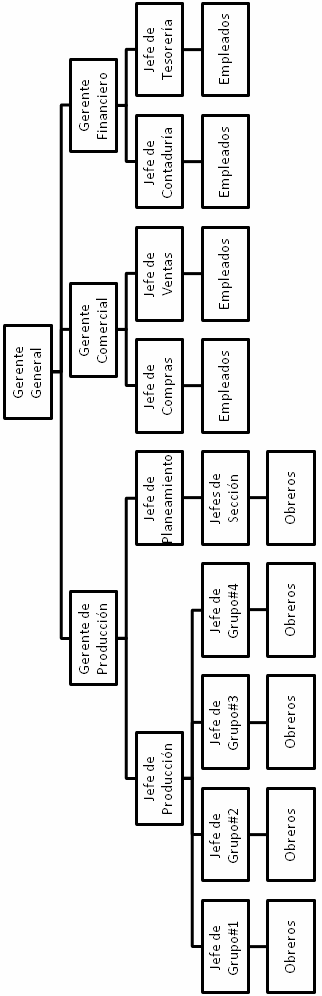
\includegraphics[scale=0.75]{images/organigrama-hercules.png}
\end{figure}

\newpage
\section{An\'{a}lisis del caso}

\subsection{Marco Te\'orico}

\subsubsection{Tipo de empresa}
La empresa fue en sus comienzos probablemente una PyME, y a medida que aument\'o su tama\~no desarroll\'o su vida como una sociedad civil. En este sentido, si bien nunca fue una empresa familiar, su estructura y organizaci\'on iniciales fueron evolucionando gradualmente a lo que es en la actualidad, probablemente provocando los problemas de planeamiento observados. Es decir, si una empresa no sufre un proceso formal de dise\~no organizacional, es altamente probable que se encuentren deficiencias en su funcionamiento a medida que pasa el tiempo y aumenta su tama\~no. Por este motivo resulta conveniente la reestructuraci\'on que se propone la empresa al contratar una consultora.

\subsubsection{Proceso de creaci\'on de valor}
Una observaci\'on interesante es el amplio proceso de conversi\'on de insumos en productos. La empresa toma como insumos materias primas muy esenciales, para utilizar en fundici\'on, carpinter\'ia, torner\'ia, moldeado, rectificaci\'on, montaje, pintura, estampado y la final instalaci\'on de los productos. Una empresa de esta complejidad necesita una estructura s\'olida y una programaci\'on muy precisa para funcionar eficientemente.

\subsubsection{Rasgos de pensamiento administrativo}
Evidentemente la empresa evolucion\'o hacia el modelo de Taylor: en un principio delegaba en los empleados parte del planeamiento de producci\'on, quienes reportaban al planeador de producci\'on, que luego completaba la programaci\'on. Esto trajo problemas por dos motivos; uno de ellos los errores de relevamiento de dichos empleados, quienes omit\'ian reportar obras paralizadas y fijaban plazos de entrega muy anticipados para tratar de compensar los retrasos en las entregas (meti\'edose en una parte de la organizaci\'on que no era su responsabilidad); el otro motivo fue el aumento de la demanda, que hizo imposible continuar con este precario sistema. Se pasa entonces a trabajar seg\'{u}n ordenes de venta, lo cual hace el negocio menos previsible (quita la posibilidad reaccionar ante fluctuaciones en el mercado, la programaci\'on se hace a medida que se vende pero no se pronostica la potencial demanda futura).

\subsection{Problema principal de la empresa}
\subsubsection{La empresa no puede enfrentar al cambio en el mercado}
El problema principal de H\'ercules surge al producirse un cambio en el mercado. La empresa comienza atendiendo a una cantidad de clientes con la cual puede trabajar en forma eficiente y c\'omoda. Al empezar a irle bien cada vez cuenta con m\'as clientes y m\'as pedidos. Esto deber\'ia serle algo muy positivo a la misma, ya que le implicar\'ia ganar m\'as que antes y ampliar su mercado. Pero esto no es lo que sucede ya que, contrario a lo que se supone como un crecimiento, es aqu\'i cuando empiezan los problemas.\\

\subsection{Consecuencias del problema principal de la empresa y sus propuestas de soluci\'on}

\subsubsection{No hay una determinaci\'on de que procesos dan valor y cuales no}
La empresa es dif\'icil de controlar y no logra una correcta planificaci\'on, debido a que su proceso productivo es muy amplio y abarcativo. De un an\'alisis de los procesos industriales de la empresa puede reconocerse una falencia: hay procesos que no agregan valor al producto final. Es decir, la empresa realiza tareas como la fabricaci\'on de las piezas a utilizar en la construcci\'on de los elevadores, las cuales podr\'ian ser compradas a terceros. Como se mencionar\'a m\'as adelante, la fabricaci\'on de las piezas tambi\'en representa un costo innecesario.
\paragraph{Soluci\'on}
Se debe determinar qu\'e procesos que agregan valor y los que no, y a partir de all\'i tomar decisiones en la direcci\'on de abandonar los procesos que no producen un beneficio a la empresa, ya sea directo o indirecto (ventajas competitivas, por ejemplo), y si este beneficio justifica el costo del proceso. Un claro ejemplo de proceso que agrega valor en la empresa es el dise\~no y construcci\'on de elevadores. Este es un trabajo que la empresa transforma directamente en ingresos, ya que es su actividad principal. Un ejemplo de proceso que no agrega valor es el de la fabricaci\'on de piezas est\'andar: ellas pueden ser compradas a un tercero, y probablemente adem\'as se reduzca su costo, ya que el tercero puede producirla en mayor cantidad, y la empresa deber\'ia podr\'ia abandonar los costos fijos asociados a su producci\'on.

\subsubsection{Grave problema de costos}
La empresa tiene un grave problema de costos, algunos de ellos ocultos tras otros problemas. Se encuentra desbordada de pedidos y no tiene una respuesta eficiente; para intentar hacerles frente a los mismos toma decisiones equivocadas y principalmente apresuradas. Intentar vender m\'as en este caso no le esta garantizando mayor ganancia ya que en alg\'un momento esta situaci\'on de toma de decisiones erroneas va a hacer que el rendimiento comience a bajar notoriamente. Las principales decisiones erroneas son:
	\begin{itemize}
 		\item Coloca personal incapacitado para ciertos puestos. 
		\item No tiene un control efectivo de lo que produce, puede estar produciendo piezas equivocadas o m\'as de lo que realmente necesita ya que no cuenta con un plan eficaz. Esto se traduce en un costo de almac\'en porque debe acumular stock de piezas.
		\item Acepta cualquier pedido sin saber si realmente llega a cumplimentarlo, por una descoordinaci\'on entre el \'area de ventas y el \'area de producci\'on.
		\item Construye cada elevador a medida del cliente lo cual perjudica la producci\'on ya que no est\'a estandarizada, lo cual hace que aumente el margen de error (costos de reparaci\'on y/o reemplazo), agrega un costo de dise\~no a cada proyecto, agrega un costo de servicio de venta personalizado, etc.
	\end{itemize}
\paragraph{Soluci\'on}
Para el problema de costos una posible soluci\'on es estandarizar los procesos de producci\'on, y establecer un nuevo proceso de selecci\'on de personal, al menos del jer\'arquico.\\
Deben dise\~narse una serie de modelos est\'andar determinando antes cu\'ales son las caracter\'isticas de los elevadores m\'as vendidos, armar un catalogo para ofrecer a los clientes y fabricar los productos en serie. De esta manera es posible disminuir al menos dos costos: el de dise\~no, que no debe repetirse para cada cliente, y el de producci\'on o compra de piezas, ya que se estandarizar\'an completamente. Con esto podr\'ia llegar a perder una parte del mercado, pero consideramos que no ser\'{a} una gran parte ya que los productos a medida en general son m\'as costosos que los est\'andar, y los productos menos costosos son los que consiguen mayor caudal de ventas.\\
Se propone que el proceso de fabricaci\'on de piezas sea tercerizado, con esto bajar\'a la dificultad del planeamiento, se tendr\'{a} un menor sector de producci\'on m\'{a}s controlable, m\'as eficiente. Disminuir\'an notablemente los costos de dep\'osito, el costo de la planificaci\'on, se reducir\'a tambi\'en el costo de las piezas, ya que al ser est\'andar habr\'a m\'as de un proveedor compitiendo con sus precios por abastecer a la empresa.\\
Para lograr este tipo de decisiones debe contratarse personal capacitado para la planificaci\'on de una empresa de la escala de H\'ercules, si es posible con experiencia en el \'area de las instalaciones en la construcci\'on, por lo menos un director o gerente de planeamiento de producci\'on que posea mayores conocimientos que los t\'ecnicos de este \'area, para poder ejercer una autoridad real. Puede establecerse un \'area de recursos humanos para definir pol\'iticas de reclutamiento apuntadas a este objetivo, o contratarse una agencia consultora de forma temporal si no se requieren tareas de RR.HH. continuas.

\subsubsection{Falta de estandarizaci\'on, diversidad de productos}
La empresa se maneja en un ambiente muy cambiante, donde las variables externas (que no son controlables) son abundantes: los productos no son est\'andar, por ello no hay plan general de producci\'on (por la particularidad de cada producto vendido); el desarrollo tecnol\'ogico de la construcci\'on var\'ia segn el lugar de instalaci\'on de cada productos, etc.
\paragraph{Soluci\'on}
La empresa necesita un vuelco hacia el enfoque de contingencias, para adaptar las variables administrativas a las externas (que no son controlables.) En este sentido, se debe verificar que el personal administrativo cuente con el alcance temporal de la discreci\'on adecuado. Se debe adem\'{a}s analizar el ambiente externo produciendo informaci\'on confiable para reducir el riesgo en la toma de decisiones. Por ejemplo, contratar una consultora, o abrir una nueva \'area de la empresa, dedicada a la estad\'istica y pron\'osticos de mercado.

\subsubsection{Contrataci\'on de personal no capacitado para las tareas requeridas}
Se nombr\'o a cargo del Planeamiento de la Producci\'on a un antiguo supervisor en 1942. El nombramiento de esta persona no cumple con los requisitos del alcance temporal de la discreci\'on. Esto quiere decir que la persona no tiene la capacidad de predecir o anticipar el desarrollo de la tarea en el lapso de tiempo adecuado para tomar decisiones de planeamiento. Esto se ve reflejado en el siguiente parrafo de la descripci\'on del caso: "Los retrasos en las entregas de elevadores hicieron que los jefes de campo fijasen los plazos de entrega muy anticipados en sus informes mensuales. Con eso las informaciones recibidas por el programador, fueron perdiendo parte de su valor como base para la programaci\'on."\ Al meter personas en lugares equivocados no se soluciona nada sino que se empeora la situaci\'on. La empresa quiza quiera ahorrarse alg\'un costo de traer a un profesional, pero a la larga tiene m\'as costo por no traerlo.
\paragraph{Soluci\'on}
Se propone situar en ese cargo a una persona que cumpla con los requerimientos que la posici\'on requiere. Alguien con experiencia y previsi\'on, que sea capaz de coordinar tiempos y tareas junto con el Area de Produccion.

\subsubsection{Conflictos entre algunas \'areas de la empresa}
"Los pedidos de los clientes tend\'ian a alcanzar l\'imites que sobrepasaban la capacidad de producci\'on de la f\'abrica. Los atrasos en la entrega de pedidos llegaron al punto de provocar serios conflictos entre los departamentos de ventas y producci\'on."
\paragraph{Soluci\'on}
Se propone incluir alg\'un tipo de nexo entre ambos departamentos. No puede pasar que el departamento de ventas y de producci\'on no se comuniquen ya que lo que se produce es lo que se vende, no se puede vender algo que no se va a poder producir. La gente de ventas no tiene el m\'as m\'inimo conocimiento de como se produce (lo cual es correcto ya que su funci\'on no es producir, sino vender) por lo que no tiene una noci\'on exacta de tiempos. Por lo que si no hay alguien que actue de nexo entre ambas \'areas, nunca va a funcionar bien. Encima una empresa vive de lo que vende por lo que este es un punto realmente importante. Creemos que ser\'ia correcto crear una relaci\'on formal entre la gerencia de ventas y la gerencia de producci\'on para que se pueda trabajar a conciencia de tiempos y no se produzcan conflictos entre ambas \'areas.

\subsubsection{Demasiadas tareas de producci\'on}
La diversificaci\'on de producci\'on produce gran parte del colapso del sistema, dado que se quiere abarcar gran cantidad de tareas de producci\'{o}n que no son pertinentes al objetivo de la empresa que es dise\~nar, construir e instalar elevadores. Sin embargo tiene la ventaja de tener capacidad de producci\'on propia y no depender de terceros, lo cual resulta interesante sobre todo cuando se trata de piezas no estandarizadas.
\paragraph{Soluci\'on}
Aqu\'i es cuando aparecen dos posibles soluciones: La primera es tercerizas la producci\'on de partes est\'andar. La contrapartida a esta soluci\'on es mejorar la programaci\'on para permitir el correcto funcionamiento del \'area de producci\'on, salvando el problema sin cerrar los talleres que producen las partes est\'andar. 
Podemos analizar los distintos costos de ambas alternativas:
Al tercerizar la fabricaci\'on debe cerrarse un \'area de la empresa, debiendo prescindir de empleados de varios niveles, o mantenerlos en otro \'area de la empresa aumentando los costos de mano de obra; se perder\'ia parte de la inversi\'on en capacidad productiva de partes est\'andar, ya que seguramente ser\'a dif\'icil vender maquinaria especializada usada. En contrapartida puede ser mejor al trabajar con un planeamiento m\'as chico, se puede tener un mejor control sobre la producci\'on verdadera de la empresa (que son los elevadores), se reduce el costo de calidad y eso puede hacer que se reduzca el costo de fabricaci\'on. No siempre al fabricar uno las piezas se garantiza el menor costo, muchas veces adquiriendolas de un tercero el mismo es menor.
El mejorar la programaci\'on conlleva costos de reorganizaci\'on en t\'erminos de personal administrativo para sostener un proceso burocr\'atico m\'as funcional que el actual; tal vez sea necesario una actualiaci\'on de los sistemas de informaci\'on de la empresa, lo cual puede ser un costo bastante alto.
Para mejorar la programaci\'on de la producci\'on podr\'ia adoptarse un cronograma como el propuesto a continuaci\'on:
\begin{enumerate}
\item Se realiza un pedido de instalaci\'on desde una obra.
\item Se analiza qu\'e partes son est\'andar y cu\'ales no (a cargo del Departamento de Ingenier\'{i}a a trav\'es del formulario de fabricaci\'on individual).
\item Las partes est\'andar se solicitan a las empresas tercerizada (por el Departamento de Compras).
	\begin{itemize}
		\item Tener en cuenta que es conveniente contar con una red de proveedores, por si uno no puede producir que otra pueda hacerse cargo de una mayor parte de la producci\'on.
	\end{itemize}
\item Teniendo en cuenta el tiempo de fabricaci\'on propio (ensamble de partes, creaci\'{o}n de las propias, etc.) m\'as el de la entrega de las partes no comunes, se elaborar\'{a} el informe para la obra.
\item En caso de par\'{a}lisis de obra, se evaluar\'{a} el tiempo del mismo, y se intentar\'ia la redistribuci\'{o}n de los semielaborados comunes en otras obras.
\item Todas las semanas se confeccionar\'an informes del avance de cada obra en que se ha encargado una instalaci\'on.
\item El Departamento de Ventas solo debe encargarse de la venta en s\'i y de los requerimientos iniciales, sin interferir en el resto del proceso.
\end{enumerate}

\section{Historia de la Empresa}
	S-S Technologies Inc. se constituy\'{o} en 1992 cuando la  compa\~{n}\'{i}a constructora y de ingenier\'{i}a integrada Sutherlaud- Schultz, de la cual formaba parte, cambi\'{o} de propietarios y los nuevos due\~{n}os vendieron la parte de SST al ex presidente de Sutherlaud- Schultz, Brock. La compa\~{n}\'{i}a era de  propiedad 100 por ciento canadiense. En \'{u}ltima instancia, SST era propiedad de su director general, Rick Brock, ex presidente de Sutherland-Schultz, y de Keith Pritchard, presidente de SST. 
	En enero de 1994 la compa\~{n}\'{i}a enfrentaba un r\'{a}pida tasa de crecimiento que se estimaba pod\'{i}a duplicarse o triplicarse en los dos a\~{n}os siguientes. En los \'{u}ltimos 3 a\~{n}os se hab\'{i}a percibido un crecimiento promedio de 33 por ciento anual y se esperaba un crecimiento de 30 a 60 o incluso 120 empleados.

	\subsection{Avance Cronol\'{o}gico de la empresa}
	\begin{enumerate}
		\item \underline{1992}. Se constituye la compa\~{n}\'{i}a al venderse la parte correspondiente a Brock. 
		\item \underline{1993}. Se perciben ingresos por 6.3 millones de d\'{o}lares.
		\item \underline{1994}. Se estima un crecimiento que duplique o triplique al del a\~{n}o anterior.
	\end{enumerate}

\section{Resumen del Funcionamiento}

	\subsection{Caracter\'{i}sticas del Sistema de Producci\'{o}n}
	\begin{itemize}
		\item La p oducci\'{o}n se divide en dos grupos: productos y sistemas integrados:
		\begin{enumerate}
			\item Productos participaba del desarrollo y venta de productos de hardware y sofware propios de la compa\~{n}\'{i}a, los cuales se vend\'{i}an por todo el mundo. Los mismos comprend\'{i}an las tarjetas simuladoras Direct-Link y el simulador PICS, los cuales peresentaban una soluci\'{o}n a un problema que ninguna otra compa\~{n}\'{i}a pod\'{i}a resolver.
			\item El grupo de sistemas integrados trabajaba en tres \'{a}reas distintas pero interrealacionadas: consultor\'{i}a, ingenier\'{i}a de sistemas y soporte a clientes brindando soluciones de calidad a problemas de hardware y software a complejos sistemas de pisos de f\'{a}bricas.
			\end{enumerate} 
		\item Ante la recesi\'{o}n, la compa\~{n}\'{i}a se ve beneficiada ya que brinda soluciones que permiten reducir los costos de automatizaci\'{o}n de las plantas y por ende los costos de producci\'{o}n.
		\item Se ten\'{i}a un enfoque de consultor\'{i}a que permit\'{i}a que quienes participaban tuvieran facultades de decisi\'{o}n y llevaba a apropiarse de los problemas y sus soluciones.
		\item Los proyectos eran asignados a individuos o equipos, seg\'{u}n el tama\~{n}o, los cuales eran autoadministrados. La responsabilidad de los proyectos reca\'{i}a en los integrantes del grupo generando un alta motivaci\'{o}n.
		\item La organizaci\'{o}n era austera, manteniendo los recursos indirectos al m\'{i}nimo.
		\item El principal recurso de la empresa lo representaba su capital humano formado de equipos muy competentes, t\'{e}cnicos y motivados. El personal t\'{e}cnico era l\'{i}der en su campo.
		\item Otro recurso era su excelente reputaci\'{o}n y relaci\'{o}n con un gran fabricante canadiense.
		\item La empresa estaba adelantada en la curva de apredizaje, habiendo enfrentado varios desaf\'{i}os, los cuales pudo resolver con \'{e}xito.
	\end{itemize}

\newpage
\section{An\'{a}lisis del caso}

	\subsection{Marco Te\'orico}

		\subsubsection{Dise\~{n}o administrativo}
			Si bien tiene un organigrama definido, la mayor parte de las relaciones que se dan en la misma son de car\'{a}cter informal. Se conforman grupos de trabajo con mecanismo coordinador de ajuste mutuo sobre los que recae la responsabilidad de las tareas que llevan a cabo. La forma de reportar no respeta el organigrama sino que se da de acuerdo a relaciones informales o costumbre.

		\subsubsection{Rasgos de pensamiento administrativo}
			La empresa presta especial atenci\'{o}n a las ciencias del comportamiento. Se busca que todos los empleados participen y sientan que todas sus necesidades se encuentran satisfechas a la vez que se valora la motivaci\'{o}n y el compromiso. Las relaciones informales cobran especial importancia con el sistema de comunicaci\'{o}n abierto que se implementa.

	\subsection{Problemas de la empresa y sus respectivas soluciones}


		\subsubsection{Falta de claridad en las metas y estrategias de la empresa}
			Los empleados no tienen en claro las metas y estrategias de la empresa. 
			Las funciones y responsabilidades de los distintos puestos resultan confusas.
			El abuso de las relaciones informales y poco respeto al organigrama genera que los empleados no reporten a quien deber\'{i}an creando caos. 
		\paragraph{Soluci\'on}
			Deber\'{i}a utilizarse un enfoque burocr\'{a}tico a fin de definir la autoridad, funciones y responsabilidades de los distintos puestos y dejar en claro la jerarqu\'{i}a de los cargos. 
			Aquellas personas en puestos de autoridad deber\'{i}an exigir que se cumplan estas relaciones. 
			Es necesario designar formalmente un gerente para el Grupo de Productos y otro para el Grupo de Sistemas Integrados. 
			Esto puede traer un conflicto interno dentro del grupo GSI  pero es necesario para resolver las confusiones que tienen los integrantes del grupo en lo que respecta a la autoridad de Shwarz respecto a Ojala.
		
		\subsubsection{Falta de espacio f\'isico}
			La compa\~{n}\'{i}a hab\'{i}a crecido tanto que resultaban insuficientes las instalaciones que compart\'{i}a con otras empresas. Como no se quer\'{i}a separar al personal, se agreg\'{o} un remolque para ubicar al personal adicional.
		\paragraph{Soluci\'on}
			Una alternativa es la b\'{u}squeda de un edificio con mayor disponibilidad de instalaciones a fin de que todos los empleados puedan trabajar en un lugar c\'{o}modo sin que sea necesaria la divisi\'{o}n del mismo. 
			Existe una segunda alternativa que es reubicar a la otra empresa del dueo de SST, SAF o esperar a la culminaci\'{o}n  o rescindir el pr\'{e}stamo con la empresa Wilson Gas. 
			La ventaja de la primera alternativa es que la empresa no tendr\'{i}a que rescindir ning\'{u}n contrato ni tratar con otra empresa. 
			Adem\'{a}s se podr\'{i}a buscar un espacio que se adecue mejor a determinadas necesidades que despu\'{e}s de a\~{n}os en la producci\'{o}n, se identifican f\'{a}cilmente. 
			Las ventajas de la segunda alternativa es que la empresa no atravesar\'{i}a una mudanza en un momento en el cual, como muestra el caso, se espera una escasez de recursos y que como consecuencia se necesitar\'{i}a que todo recurso existente este abocado a satisfacer las necesidades del mercado sin perder tiempo en una mudanza.

		\subsubsection{No hay una figura que realice una tarea de recursos humanos}
			No se registran las evaluaciones de desempe\~{n}o y no existe una figura a la cual se le puedan hacer consultas referidas a los l\'{i}mites salariales de los diversos puestos.
		\paragraph{Soluci\'on}
			Creaci\'{o}n de un \'area de recursos humanos para que pueda guardar registro de las evaluaciones de desempe\~{n}o y que adem\'{a}s sirva para que los empleados puedan hacer consultas no t\'{e}cnicas sin sentirse inc\'{o}modos por tener que realizar la consultar a un superior.  

		\subsubsection{Falta de incentivo salarial a los empleados}
			Conflicto generado por ausencia de bonos y compensaciones. Los empleados no tienen un incentivo o un dinero extra por el trabajo realizado, con lo cual esto puede generar conflictos futuros (y no tan futuros) con los empleados.
		\paragraph{Soluci\'on}
			Se propone que la empresa realice evaluaciones individuales de performance del personal. 
			Para esto es necesario que se defina y respete un organigrama a fin de que quede en claro qui\'{e}n estar\'{a} siendo evaluado por qui\'{e}n. 
			Los mismos solo deberan premiar un excelente desempe\~{n} y preferentemente ser entregados a equipos de personal a fin de fomentar la cooperaci\'{o}n y limitar la competencia interpersonal. 
			Tambi\'{e}n debe considerarse entregar premios adicionales por contribuciones excepcionales.
			Los gerentes de cada \'{a}rea notificar\'{i}an al \'{a}rea de recursos humanos de los resultados de las evaluaciones t\'{e}cnicas para que este \'{a}rea sea la encargada de entregar los bonos y premios.
			Sera una funci\'{o}n del \'{a}rea de recursos humanos estudiar el estado econmico de cada empleado para analizar si es viable dar en forma de bonificaci\'{o}n acciones de la empresa para poder aumentar el sentimiento de pertenencia que siente cada empleado.


		\subsubsection{R\'apido crecimiento}
			Inminente crecimiento de la empresa en el corto plazo. La empresa en un per\'iodo corto de tiempo implement\'o un crecimiento importante, el 				cual fue demasiado r\'apido e hizo que se deban adaptar muchas cosas, algunas en forma eficiente y otras en forma ineficiente.
		\paragraph{Soluci\'on}
			Considerando que la empresa cuenta con mano de obra muy calificada es necesario ir contratando empleados para poder capacitarlos adecuadamente. 
			Teniendo en cuenta que la capacitaci\'{o}n implica que los empleados actuales destinen horas de producci\'{o}n e investigaci\'{o}n a la capacitaci\'{o}n de los nuevos empleados, la contrataci\'{o}n de personal deber\'{a} hacerse de a poco para que la producci\'{o}n no se vea comprometida.

\documentclass[12pt,a4paper,spanish]{article}
\usepackage[spanish]{babel}

\usepackage[ansinew]{inputenc}


\usepackage{graphicx}
\usepackage{float}
\usepackage{array}
	  \oddsidemargin 0in
      \textwidth 6.75in
      \topmargin 0in
      \textheight 10.0in
      \parindent 0em
      \parskip 2ex
\usepackage{anysize}
\marginsize{3cm}{2cm}{1.0cm}{1.0cm}

\pagestyle{plain}

\begin{document} 
\title{
\begin{table}[!h]
	\begin{tabular}{m{2cm}m{15cm}}
		\multicolumn{1}{l}{}
		 
\includegraphics[scale=0.5, bb=0 0 0 0]{logo-fiuba.png} & 
		 \begin{center}
		 	\begin{LARGE}
				Universidad de Buenos Aires	\linebreak \linebreak		 							Facultad de Ingenier\'{i}a  \linebreak \linebreak
				7112 - Estrucutra de las Organizaciones \linebreak \linebreak
				2do. Cuatrimestre de 2009
			\end{LARGE}
		 \end{center}\\
\end{tabular}
\end{table}
\begin{Large}
 \begin{center}
		\underline{An\'{a}lisis Caso Ford} \linebreak \linebreak
        Grupo Nro:	R2
\end{center}
\end{Large}
}
\date{}
\maketitle

\thispagestyle{empty}

\author{
\begin{Large}
\begin{center}
		\underline{Integrantes}  \linebreak 
\end{center}
\end{Large}
\begin{center}
	\begin{tabular}{|| c | c | c ||}
		\hline
		\begin{large}Apellido,Nombre\end{large} & 
		\begin{large}Padr\'{o}n Nro.\end{large} & 
		\begin{large}E-mail\end{large}\\
		\hline
		Bruno Tom\'as & 88.449 & tbruno88@gmail.com\\
		\hline
		Chiabrando Alejandra Cecilia & 86.863 & achiabrando@gmail.com\\
		\hline
		Fern\'{a}ndez Nicol\'{a}s  & 88.599 & nflabo@gmail.com\\
		\hline
		Invernizzi Esteban Ignacio & 88.817 & invernizzie@gmail.com\\
		\hline
		Medbo Vegard & \- & vegard.medbo@gmail.com\\
		\hline
		Meller Gustavo Ariel & 88.435 & gustavo\_meller@hotmail.com\\
		\hline
		Mouso Nicol\'as & 88.528 & nicolasgnr@gmail.com\\
		\hline
		Mu\~noz Facorro Juan Mart\'in & 84.672 & juan.facorro@gmail.com\\
		\hline
		Wolfsdorf Diego & 88.162 & diegow88@gmail.com\\
		\hline
	\end{tabular}
\end{center}
}

\newpage
\setcounter{page}{1}
\tableofcontents

\newpage

\section{Introducci�n}
	Para el �xito de una empresa, es indispensable que �sta conozca su ambiente y se sepa adaptar al mismo.
	No basta �nicamente con cerrar tratos convenientes con los clientes, sino que tambi�n hace falta considerar otras variables, como por ejemplo los proveedores y la competencia.
	El conjunto de todas estas variables forma lo que se conoce como el ambiente.

	Formalmente, el ambiente se puede definir como el sistema de nivel superior en el que se inserta la empresa y est� formado por aquellos factores, fuerzas o variables que influyen directa, o indirectamente, en los procesos de gesti�n\cite{ITE}.
	El conocimiento de una empresa de su ambiente le permite explotar al m�ximo su potencial e incluso poder anticiparse a situaciones riesgosas.

	La empresa Ford Motor Company  se fund� a principios del siglo XX.
	Ya desde sus comienzos se dedic� a la producci�n de autom�viles.
	Mediante la instalaci�n de cintas de ensamblaje r�pidamente consigui� volverse altamente competitiva y de esta forma se hizo un lugar en el mercado.

\section{Cambios en la administraci�n del ambiente}
	\begin{enumerate}
		\item{\emph{Suministro de partes por parte de proveedores:}} se agregaba valor mediante el ensamblaje de las piezas.
		\item{\emph{Integraci�n vertical:}} comienzo de fabricaci�n de las piezas necesarias previas al ensamblaje.
		\item{\emph{Potenciales proveedores m�s eficientes:}} fin de modelo verticalmente integrado. Vuelta a comprar las piezas a proveedores eficientes.
		\item{\emph{Irrupci�n en el mercado por parte de competencia externa:}} adquisici�n de porcentajes en las empresas de proveedoras.
	\end{enumerate}
	
\section{An�lisis}
	\subsection{Suministro de partes por parte de proveedores}
		La innovaci�n de la Ford Motor Company en sus inicios, fue la aplicaci�n de una cinta de ensamblaje m�vil.
		La utilizaci�n de esta cinta le permit�a tener una capacidad de producci�n muy grande, que no necesariamente pod�a cubrir con la propia producci�n de los insumos que necesitaba.
		No depender de los proveedores, por los problemas de calidad e incompatibilidad entre proveedores que ellos conllevan, no era tan importante como captar el mayor porcentaje del mercado automotriz incipiente.
		Por esta raz�n, se acord� con determinados proveedores para poder obtener los insumos necesarios para satisfacer la demanda en el mercado.

		El problema que surg�a de este modelo era que el proceso de producci�n se hac�a muy largo.
		Cada vez que las piezas de un proveedor eran incompatibles con las de otro proveedor, se demoraba la producci�n hasta hacer los ajustes necesarios que permitieran la compatibilidad entre las piezas.
		Era necesario tener la producci�n fuertemente estandarizada para evitar estas situaciones y tener un documento en el cual ampararse al momento de hacer los reclamos a los proveedores: los contratos de suministro.

		No obstante, para explotar la ventaja comparativa que ten�a por sobre otras empresas automotrices, la tecnolog�a de la cinta de ensamblaje m�vil, era necesario un manejo del ambiente con caracter�sticas similares a estas.

	\subsection{Integraci�n vertical}
		Una vez ya consolidada en el mercado, la Ford Motor Company crey� prioritario no descuidar la calidad de sus productos.
		Al no poder cambiar directamente la calidad de sus insumos ya que estos eran producidos por sus proveedores, decidi� fabricarlos por s� misma.
		Esta integraci�n vertical se realiz� de dos formas: por un lado, se tom� el control de las empresas de algunos proveedores y por otro, se comenzaron operaciones propias para la producci�n de los insumos necesarios.
		As� fue que, por ejemplo, compr� minas para la extracci�n de hierro, lo transport� a sus plantas donde fabric� acero y luego lo us� para la manufactura de la carrocer�a y otras piezas.

		La integraci�n vertical le permit�a no depender de otras organizaciones para satisfacer la demanda del mercado.
		La posici�n de Ford ahora le permit�a poder satisfacer por s� misma un aumento en la demanda.
		Adem�s, hab�a alcanzado un poder adquisitivo que le permit�a tomar el control de otras empresas.

		No es un detalle menor la depresi�n econ�mica que atraves� Estados Unidos en la d�cada del 30�, la cual probablemente provoc� la quiebra de algunos de los proveedores, haciendo que estos no puedan cumplir los compromisos que ten�an hacia Ford. 
		Para esta empresa, la integraci�n vertical era una salida para no verse arrastrada junto a algunos de sus proveedores.

	\subsection{Potenciales proveedores m�s eficientes}
		Sin embargo, la producci�n de sus insumos result� ser demasiado costosa.
		El excesivo tama�o que hab�a adquirido Ford hac�a que aparezcan problemas de comunicaci�n.
		Mientras tanto, aparec�an potenciales proveedores que demostraban ser m�s eficientes en la producci�n de los insumos que Ford necesitaba, dando lugar a una oportunidad para reducir los costos de los insumos.
		Adem�s, la situaci�n econ�mica mundial hab�a cambiado nuevamente y en la d�cada del �50 se esperaba nuevamente una �poca de estabilidad.

		Por estas razones, Ford decidi� volver a acordar con proveedores para el suministro de materia prima.
		La alta participaci�n que tenia Ford en el mercado le permiti� poder negociar precios favorables al momento de establecer las condiciones del acuerdo.
		De esta forma logr� obtener ventajas sobre General Motors que segu�a con un modelo basado en la integraci�n vertical y sufr�a problemas similares a los de Ford.

	\subsection{Irrupci�n en el mercado por parte de competencia externa}
		Durante varias d�cadas, la competencia que sufr�a Ford era solo competencia interna por parte de Chrysler y General Motors.
		Esta competencia no era destructiva ya que las empresas acordaban informalmente pol�ticas de precios, estableciendo de esta manera un oligopolio en la industria automotriz.
		Cada una de las empresas ten�a un sector del mercado y su porcentaje dentro de �ste no sufr�a grandes variaciones.
		Sin embargo, en la d�cada de 1980, la industria japonesa logr� ser suficientemente competitiva para ingresar en el mercado estadounidense.

		Las empresas japonesas contaban con determinadas t�cnicas que les permit�an obtener ventajas comparativas sobre las estadounidenses:
		\begin{itemize}
			\item{\emph{Participaci�n en los proveedores:}}
				Mediante la tenencia de acciones de las empresas proveedoras, las empresas japonesas lograban incidir en el control de estas sin llegar a tener los problemas de comunicaci�n y escala que Ford hab�a sufrido cuando se hab�a integrado verticalmente.

			\item{\emph{Sistema de Inventario Justo a Tiempo (JIT):}}
				Es una t�cnica implementada inicialmente por Toyota que consiste en reducir el costo de la gesti�n y reducir las p�rdidas que ocurren debido a contar con stocks innecesarios.
				No se produce bajo suposiciones, sino bajo pedidos concretos.
				Por lo tanto, se reducen los costos de almacenamiento.
				La aplicaci�n de esta t�cnica ha generado un aumento en la productividad de las empresas que la utilizaron.

			\item{\emph{Keiretsu:}}
				El keiretsu es un tipo de modelo empresarial donde existe una coalici�n de empresas unidas bajo determinados intereses.
				La ventaja de este tipo de modelo es que en estas coaliciones suele haber organizaciones que pueden ayudar en la parte financiera de la producci�n, como por ejemplo bancos.
				Un ejemplo de Keiretsu es Mitsubishi, que actualmente maneja el banco Mitsubishi UFJ.

			\item{\emph{Investigaci�n:}}
				La investigaci�n se realizaba entre varias empresas y con la colaboraci�n del gobierno.
				De esta forma, la investigaci�n produc�a, con menores costos individuales, mayores resultados que, a pesar de tener que ser compartidos entre algunas empresas, permit�an obtener una ventaja comparativa sobre las empresas que no formaban parte del grupo de colaboraci�n.

		\end{itemize}

		Estas t�cnicas fueron, algunas en mayor medida que otras, copiadas por Ford.
		Una de las medidas al adoptar estas t�cnicas fue comprar acciones de algunos de sus proveedores (Cummings, Excel Industries y Decona).
		Como ya se mencion� anteriormente, esto le permiti� tener una cuota de control sobre el accionar de sus proveedores.
		Otra medida fue diversificarse en el mercado, logrando comprar el 49$\%$ de la compa��a de alquiler de autos Hertz, donde adem�s de obtener ganancias por medio del negocio de la empresa en s�, consigui� publicidad y colocaci�n de sus autos ya que gran parte de los que se alquilan, son producidos por la Ford Motor Company.
		En lo que respecta a la investigaci�n, Ford se asoci� con otros competidores para financiar un programa de investigaci�n conjunta y desarrollar nuevos productos.

\section{Paralelismo entre Ford y las empresas japonesas}
Como mencionamos anteriormente uno de los problemas que le aparecen a Ford es la irrupci�n en el mercado por parte de competencia externa, en este caso empresas japonesas. A partir de ahora detallamos el paralelismo entre lo hecho por Ford y lo hecho por las empresas japonesas, para intentar ver las diferencias entre ambos.
	\subsection{Visi�n adelantada}
	Las empresas japonesas fueron precursoras y mediante un estudio de mercado implementaron diversas ideas las cuales le resultaron muy favorables. La gran ventaja es que lo hicieron antes que todo el resto de las empresas mundiales con lo cual se les anticipar�n y les ganaron terreno. En esto tambi�n le ganan a Ford, ya que es una empresa de Estados Unidos. 
	\subsection{Diferencias de pensamiento}
	Las f�bricas japonesas se aliaban con los proveedores, ya que ten�an el pensamiento de que si a una le iba bien a la otra tambi�n le iba a ir bien. Con una buena cooperaci�n entre ambas partes, ambas crecer�an a la par. En Norteam�rica la relaci�n entre proveedores y f�bricas no era as�. Se ten�a un pensamiento de que hab�a que tratar de obtener la mayor ventaja posible sobre el otro, es decir, cuanto m�s se le pod�a sacar al otro mejor. Este es un pensamiento totalmente erroneo y es uno de los puntos m�s importantes en los cuales los japoneses ganaron terreno. Supieron dejar de lado diferencias y rencores entre empresas dandose cuenta de los beneficios que les pod�a traer y en eso fueron muy inteligentes.
	\subsection{Implementaci�n err�nea de los m�todos japoneses}
	Al ver como en Jap�n las cosas funcionaban bien, en Norteam�rica se los quizo imitar. Las f�bricas Norteam�ricanas intentaron aliarse con los proveedores, pero no como deb�an. En vez de producir una alianza terminaban comprando a los proveedores con lo cual se produj� una integraci�n vertical, lo cual no les serv�a absolutamente para nada, no mejoraban ya que ten�an m�s cosas para producir y no se dedicaban precisamente a lo que ellos produc�an. Ah� se ve el error grave cometido. Si se quiere imitar algo, se debe hacer en forma correcta, no a las apuradas y mal.
	\subsection{Diferencias culturales}
	Para la gente de Jap�n es un orgullo ver que la empresa en la que uno trabaja le va bien. Los japoneses tienen una forma distinta de ver las cosas. Se pueden quedar horas extra trabajando en conjunto para mejorar sus empresas, sin importarles que les den o no dinero extra. El orgullo que ellos tienen por ver que lo que hacen sale bien, es una gran satisfacci�n. En Norteam�rica (y en gran parte del mundo) no sucede as�. Los empleados no ven la hora de que termine su d�a de trabajo, no les interesa que la empresa crezca (hasta algunos quieren que a su empresa le vaya mal, sin darse cuenta de que su empleo depende de ello) y por cada segundo extra que trabajen van a exigir que se les pague. Hay como una ley de que si no se les paga extra no se trabaja extra. Esto es una de las cosas m�s dificiles de cambiar ya que una cultura no se cambia de un d�a para el otro. Esto puede llevar a\~nos o siglos en implementarse.

\newpage
\begin{thebibliography}{9}
	\bibitem{ITE} 	Innovaci�n Tecnologica en las Empresas. \\
					Sa�z Vacas, Fransisco; Garcia, Oscar; Palao, Javier; Rojo, Pedro.
	\bibitem{Wikipedia} Wikipedia EN.
\end{thebibliography}

		
		

\end{document}


\part{An�lisis de Empresa}

\chapter{Marsans Argentina}

\section{Comparaci\'{o}n y Elecci�n de Empresas}

\subsection{Marsans}

\subsubsection{Disponibilidad}
Nicol\'{a}s Fern\'andez, uno de los integrantes de nuestro grupo trabaj\'{o} en la empresa alrededor de dos a\~nos. Eso hizo que forme una buena relaci\'{o}n con algunos de los integrantes de la misma. Hablando con uno de los gerentes le coment\'{o} la idea de trabajar con Marsans Argentina S.A. a lo que el gerente le comunic\'{o} que no habr\'{i}a ning\'{u}n problema, que simplemente avisando con un peque\~no tiempo de anticipaci\'on, de no m\'{a}s de 2 o 3 d\'{i}as, podr\'{i}amos concretar las entrevistas o recavar la informaci\'on necesaria por medios electr\'onicos. Esto nos di\'{o} una pauta de que la disponibilidad es muy buena y que la empresa tiene la predisposici\'{o}n que necesitamos, aunque con una peque\~na demora, por lo cual el puntaje elegido fue un 8.

\subsubsection{Contacto}
Nicol\'{a}s Fern\'andez tiene contacto directo con: Sonia Kraimer (Gerencia de Recursos Humanos) y Alejandro Zubiria (Supervisor de Sistemas), con los cuales mantiene una muy buena relaci\'{o}n. A su vez conoce a distintas personas de otras \'{a}reas y tambi\'{e}n a trav\'{e}s de estas dos personas mencionadas puede obtener el contacto con cualquier otra persona que se necesite, en cualquier nivel jer\'arquico. Los contactos de la empresa nos parecieron muy predispuestos y creemos que vamos a poder acceder a cualquier contacto de otra \'{a}rea con lo cual el puntaje elegido fue un 10.

\subsubsection{Estructura}
La empresa es reconocida dentro del pa\'{i}s. La misma cuenta con un organigrama formal. Tiene diversos departamentos, sectores y puestos en los que se delegan responsabilididas y disminuye progresivamente la autoridad formal. Esto resulta una estructura ideal para el proyecto que realizaremos. El puntaje elegido fue un 10.

\subsubsection{Conocimiento de la Estructura}
Los contactos que tenemos en la empresa tienen amplio conococimiento acerca de la estructura, al igual que Nicol\'{a}s Fern\'andez, quien trabaj\'{o} all\'{i} en el \'area de Sistemas, que asiste al funcionamiento de todas las dem\'as, con lo cual se tiene un conocimiento bastante vasto sobre la misma y el hecho de que un integrante del grupo la conozca nos resulta muy \'{u}til. El puntaje elegido fue un 9.

\subsubsection{Ubicaci\'{o}n}
La empresa se encuentra en Suipacha y Avenida Santa F\'{e}, muy cerca del centro de la ciudad con lo cual se puede llegar cas\'{i} desde cualquier punto y queda relativamente cerca de ambas sedes de la facultad, tanto Las Heras como Paseo Col\'{o}n. A pesar de que no todos los integrantes vivimos en la Ciudad de Bs. As., estamos de acuerdo en que la ubicaci\'{o}n es excelente al estar en plena ciudad y tener muy f\'{a}cil acceso y abundantes medios de transporte desde y hacia cualquier ubicaci\'on. El puntaje elegido fue un 10.

\subsubsection{Tama\~{n}o}
La empresa cuenta con alrededor de 70 empleados, con lo cual el n\'umero se encuentra dentro del rango \'optimo sugerido por la c\'atedra y nos parece un buen n\'{u}mero al no ser muy grande ni muy chico. El puntaje elegido fue un 10.

\subsection{Software Factory, SAP y Consultor\'{i}a}
\subsubsection{Disponibilidad}

Uno de los integrantes del grupo que presenta este informe trabaja actualmente en la empresa referida. A pesar de no ser una empresa que supere los 200 empleados, la actitud que se percibe de la gerencia es altamente burocr\'{a}ctica. Es por esta raz\'{o}n que a pesar de tener una buena relaci\'{o}n con el gerente del \'{a}rea de Software Factory, la posibilidad de obtener entrevistas o informaci\'{o}n sobre la empresa se ve sujeta a la buena voluntad de las otras partes involucradas, lo cual es poco menos que una seguridad, si lo que se quiere es una alta disponibilidad. Es por esto que el puntaje asignado a este aspecto es 7.

\subsubsection{Contacto}

El contacto principal, como se mencion\'{o} anteriormente, es el gerente del \'{a}rea de Software Factory, con el cual se tiene una muy buena relaci\'{o}n laboral y personal. Se podr\'{i}a recurrir tambi\'{e}n a la ayuda de contactos en el \'{a}rea de recursos humanos y finanzas para la obtenci\'{o}n de informaci\'{o}n, aunque ya no en el nivel gerencial, lo cual agilizar\'{i}a el proceso de consulta pero limitar\'{i}a el acceso al tipo de datos que se pueden conseguir. El puntaje asignado a este aspecto es 8.

\subsubsection{Estructura}

Luego de la compra de una empresa dedicada al servicio de consultor\'{i}a SAP y la venta de un data center, se produjo una importante reforma en la estructura de la empresa, la cual incluyo recortes de personal, tanto a nivel gerencial, como administrativo y operativo. El nuevo organigrama fue dado a conocer a todos los empleados, por lo cual \'{e}ste se encuentra disponible para los objetivos de este informe. El puntaje asignado a este aspecto es 9.

\subsubsection{Conocimiento de la Estructura}

A pesar de estar disponible el nuevo organigrama, el conocimiento de la estructura real de la empresa no es muy profundo, dado que la re-estructuracion tuvo lugar recientemente por lo que el funcionamiento del \'{a}rea de SAP y las consultor\'{i}as relacionadas se ignoran. Esta l\'{i}nea de negocios es una de las m\'{a}s grandes que tiene actualmente la empresa, por lo tanto se desconoce la estructura de un porcentaje importante de la misma. El puntaje asignado a este aspecto es 6.

\subsubsection{Ubicaci\'{o}n}

Las oficinas se encuentran distribuidas entre un edificio en San Telmo, cerca de la Facultad de Ingenier\'{i}a, y otro en Mart\'{i}nez, zona norte del Gran Buenos Aires. En la sede de San Telmo funciona la Software Factory y el Call Center, mientras que en Mart\'{i}nez se desarrollan las actividades de SAP y consultor\'{i}a. El puntaje asignado a este aspecto es 10.

\subsubsection{Tama\~{n}o}

El n\'{u}mero de empleados, teniendo en cuenta todas las l\'{i}neas de negocios, se encuentra entre 150 y 200, con lo cual seg\'{u}n los par\'{a}metros establecidos por la c\'{a}tedra se encuentra dentro del n\'{u}mero deseado, aunque ser\'{i}a un poco grande si la estimaci\'{o}n obtenida es inexacta y la realidad supera el m\'{a}ximo considerado. El puntaje asignado a este aspecto es 8. 

\subsection{Constructora: Obras Ferroviarias}
\subsubsection{Disponibilidad}

Esta empresa parece estar en un constante ambiente de cambio y necesitar de un constante control y coordinaci\'{o}n de las tareas a realizar, por lo que el tiempo que pueden ofrecer los empleados es bastante reducido. El puntaje asignado a este aspecto es 6.

\subsubsection{Contacto}

La hermana de uno de los integrantes del grupo que presenta este informe trabaja en la empresa como secretaria tanto del gerente de Administraci\'{o}n y Finanzas, como del gerente de Producci\'{o}n. A pesar de ser este un contacto s\'{o}lido y seguro, la informaci\'{o}n quiz\'{a}s m\'{a}s sensible y espec\'{i}fica, queda fuera de su alcance por lo que habr\'{i}a que recurrir a la gerencia la cual, como se menciona en el punto anterior, dispone de muy baja disponibilidad. El puntaje asignado a este aspecto es 6.

\subsubsection{Estructura}

El organigrama de la empresa ha sido solicitado varias veces, pero el mismo nunca fue, al d\'{i}a de la fecha, confeccionado e informado a sus empleados. Parecer\'{i}a que el nivel de desorganizaci\'{o}n que se deduce de los comentarios del funcionamiento de la empresa, est\'{a} fuertemente ligado con el hecho de que \'{e}sta carece de una estructura formal que le permita mejorar su rendimiento. El puntaje asignado a este aspecto es 5.

\subsubsection{Conocimiento de la Estructura}

La informaci\'{o}n disponible sobre la estructura formal de la empresa es casi nula incluso para sus propios empleados, lo que marca una tendencia desfavorable a la hora de considerarla como sujeto de an\'{a}lisis. El puntaje asignado a este aspecto es 5.

\subsubsection{Ubicaci\'{o}n}

Las oficinas administrativas est\'{a}n localizadas en Retiro, en las que se puede encontrar a la gerencia de la empresa, por ende donde se concentra la mayor cantidad de informaci\'{o}n relevante para este informe. El puntaje asignado a este aspecto es 8. 

\subsubsection{Tama\~{n}o}

La cantidad de empleados asciende a m\'{a}s de 400, incluyendo, adem\'{a}s del personal administrativo, el operativo y el de obra. Debido a que este n\'{u}mero sobrepasa los l\'{i}mites sugeridos, el puntaje asignado a este aspecto es 4.

\subsection{Servicios e Intrumentaci\'{o}n para el Control Ambiental Industrial}
\subsubsection{Disponibilidad}

Debido a una auditor\'{i}a por la que debe pasar la empresa, el tiempo del que disponen los empleados es reducido, ya que de la aprobaci\'{o}n de esta auditor\'{i}a depende la retenci\'{o}n de su cliente m\'{a}s importante. A pesar de esto, la empresa estar\'{i}a dispuesta a brindar todo tipo de informaci\'{o}n. El puntaje asignado a este aspecto es 8.

\subsubsection{Contacto}

El hijo del due\~{n}o de la empresa, el cual trabaja en el \'{a}rea de Comercializaci\'{o}n de \'{e}sta, es un amigo muy cercano de unos de los integrantes del grupo que presenta este informe. Esta relaci\'{o}n asegura la buena voluntad por parte de la empresa de ayudar, en la medida que le sea posible, con cualquier tipo de informaci\'{o}n necesaria. El puntaje asignado a este aspecto es 8.

\subsubsection{Estructura}

Como resultado de la auditor\'{i}a a la que es sometida, se est\'{a}n realizando cambios estructurales y de procesos en la empresa, por lo cual, podr\'{i}a decirse que un an\'{a}lisis que se haga en esta situaci\'{o}n posiblemente resultar\'{i}a ambiguo y poco \'{u}til. El puntaje asignado a este aspecto es 6.

\subsubsection{Conocimiento de la Estructura}

La informaci\'{o}n que se tiene sobre la actual estructura de la empresa es obsoleta, debido al ya mencionado proceso de re-estructuraci\'{o}n al cual est\'{a} siendo sometida. El puntaje asignado a este aspecto es 5.

\subsubsection{Ubicaci\'{o}n}

Cuenta con oficinas en el barrio de Belgrano, donde se encuentran las oficinas centrales de la empresa, y otras en la provincia de Neuqu\'{e}n, las cuales no ser\'{i}an accesibles para los fines de este informe. El puntaje asignado a este aspecto es 7.

\subsubsection{Tama\~{n}o}

La empresa en su totalidad cuenta con 20-30 empleados, distribu\'{i}dos entre las dos oficinas mencionadas en el punto anterior. El puntaje asignado a este aspecto es 5.

\subsection{Tabla Comparativa}

\small
\begin{center}
\begin{tabular}{|| c | c | c | c | c | c | c ||}
\hline
\hline
T\'{e}rminos & Peso & Soft.Fact. & Marsans & Obras Ferr. & Sist.Ctrl.Adm. & Manuf. Avellaneda\\
\hline
Disponib.  & 10 & 7 & 8 & 6 & 8 & 8 \\
\hline
Contacto   & 10 & 8 & 10 & 6 & 10 & 10 \\
\hline
Estructura & 9 & 9 & 10 & 5 & 6 & 8 \\
\hline
Conoc. Estr. & 9 & 6 & 9 & 5 & 5 & 10 \\
\hline
Ubicaci\'{o}n & 8 & 10 & 10 & 8 & 7 & 5 \\
\hline
Tama\~{n}o   & 7 & 8 & 10 & 4 & 5 & 10 \\
\hline
\hline
Totales & - & 421 & 521 & 302 & 370 & 452 \\
\hline

\end{tabular}
\end{center}

\subsection{Justificaci\'{o}n de la Selecci\'{o}n de la Empresa}

Una vez hecha la tabla de comparaci\'{o}n con todos los items que cre\'imos importantes, la empresa que sum\'o el mayor puntaje fue Marsans Argentina S.A.
Al elegir los pesos de la tabla de comparaci\'{o}n, en lo que m\'as \'enfasis se puso fue tanto en la disponibilidad como el contacto, teniendo un segundo plano la estructura y el conocimiento de la estrucutra y siendo las caracter\'isticas con menor relevancia, la ubicaci\'on y el tama\~no.
Marsans obtuvo puntajes similares para casi todos los items a evaluar a diferencia de las dem\'{a}s empresas, en las cuales fueron muy variados los puntajes; algunas con puntajes muy altos para algunos items y muy bajos para otros y otras teniendo una regularidad de puntajes en todos los items, pero siendo estos bajos.
En s\'{i}ntesis Marsans Argentina S.A. nos pareci\'{o} la empresa que mejor se puede amoldar al trabajo que debemos realizar y creemos que vamos a poder tener toda la informaci\'{o}n que necesitemos de la misma cuando la requerramos.
A continuaci\'{o}n detallamos el porque de la elecci\'{o}n de los puntajes de cada item en particular, con una breve explicaci\'{o}n de cada uno.

En s\'{i}ntesis creemos que la empresa elegida es la mejor para lo que vamos a tener que trabajar. La misma cuenta con todo lo pedido y esperamos que la elecci\'{o}n de la misma confirme a lo largo del trabajo que es la opci\'on m\'as adecuada para el mismo, por todo lo planteado en este documento.

\section{Historia de la Empresa}

\subsection{Escenario mundial}

En 1910 naci� en Barcelona, bajo el nombre de Viajes Marsansrof, y es la agencia de viajes pionera en Espa�a. Posteriormente pas� a denominarse Viajes Marsans, agencia de viajes mayorista-minorista.
Viajes Marsans es una compa��a din�mica y en claro proceso de expansi�n, que ya en el a�o 2000 contaba con 400 Agencias de Viajes, entre propias y asociadas, y en la actualidad cuenta con m�s de 550 Agencias de Viajes distribuidas por toda la geograf�a nacional.
Adem�s, Viajes Marsans est� integrada en el Grupo Marsans por lo que est� ligada a las principales mayoristas de viajes, empresas de transportes por carretera, compa��as a�reas, etc.
La historia de Viajes Marsans est� indudablemente unida al origen y desarrollo de un gran grupo: El Grupo Marsans.
Todas las empresas del grupo forman una gran familia, que a�na a diversos sectores y que contin�a en su expansi�n y crecimiento continuo.


\subsection{Escenario local}

Marsans Argentina es una filial del Grupo Marsans, el cual tiene alrededor de 100 a�os de presencia en el mundo. Este nombre estuvo por mucho tiempo en vigencia como la agencia de viajes de referencia en Espa�a y varios pa�ses de Sudam�rica. En Argentina en particular, tuvo mucho �xito durante muchos a�os ya que ten�a el respaldo del Grupo. Durante la convertibilidad peso-d�lar, la empresa manejaba un monoproducto que era la venta de vuelos charter con hoteler�a al caribe. Al abandonar nuestro pa�s este modelo econ�mico, la empresa debi� cambiar de negocio dado que el que llevaban dej� de ser viable. El poder adquisitivo de la poblaci�n local disminuy� respecto a los precios de los productos tur�sticos extranjeros; al ocurrir esto, la empresa propuso como objetivo ampliar sus operaciones a una empresa mayorista de tipo emisivo y receptivo, abriendo los departamentos de ventas internacionales, nacionales y receptivo.

Estos nuevos departamentos evolucionaron positivamente hasta el principios del 2008 donde comenz� la crisis institucional en Argentina y comenzaron a sentirse los efectos de la crisis financiera mundial. La primera afect� directamente al negocio de venta de paquetes tur�sticos, tanto de viajes dentro de la Argentina como hacia el exterior. La segunda golpe� el principal mercado receptivo con el que trabajaba la empresa, el espa�ol, lo cual hizo que este negocio se vea seriamente afectado.

Es por esto que la empresa entr� en un proceso de reestructuraci�n imprevisto y no planificado, reduciendo personal y recursos, pasando de emplear a 120 personas a alrededor de 40 el d�a de hoy. La ca�da abrupta en las ventas gener� un problema financiero grave, llevando a la empresa a la necesidad de vender, en algunos casos, por debajo de los costos, con la intenci�n de obtener liquidez. Para lograr obtener esta �ltima se potenci� el negocio de venta de pasajes a�reos. Algunos de los mercados extranjeros en los que trat� de incursionar sin �xito fueron China e India. En ambos destinos se invirti� dinero en marketing y publicidad, sin obtener pr�cticamente retorno alguno. En este proceso de reestructuraci�n tambi�n se pas� de disponer de dos plantas de un edificio a contar con una sola, reduciendo considerablemente el espacio de trabajo.

Es en esta situaci�n de crisis que el Grupo Marsans necesita de los servicios de una consultora para que analice la estructura de su filial en Argentina, con el fin de poder llevar adelante un plan de salvataje.



\section{An�lisis}

\subsection{Introducci�n}

Frente a la crisis, la empresa implement� decisiones que buscaban soluciones en el corto plazo de problemas puntuales sin implementarse pol�ticas para el largo plazo. Se llevaron adelante importantes reducciones de personal que hicieron que la estructura de la empresa se fuera desdibujando y resultara inconsiste con el organigrama que se ten�a, el cual, a pesar de esto, nunca fue actualizado. Algunas �reas quedaron sobrecargadas al tiempo que otras quedaron con poco trabajo. Asi mismo, las funciones del personal comenzaron a quedar poco claras al no redefinir las funciones de los puestos luego del recorte y las relaciones informales comenzaron a predominar por sobre las formales llevando a problemas de comunicaci�n entre las gerencias. A continuaci�n, se presenta un an�lisis detallado de los principales problemas que se encontraron.

\subsection{Identificaci�n de los Principales Problemas}

El problema principal es una pobre conducci�n y la falta de una estrategia claramente definida. Nos referimos a estrategia como un grupo de personas capacitadas, organizadas en una estructura adecuada, que busca aplicar la tecnolog�a disponible para desarrollar los procesos requeridos por la empresa.

En cuanto a la organizaci�n del trabajo dentro de la empresa, lo que primero se destaca es la dimensi�n del estrato gerencial, la cual se encuentra desproporcionada respecto al personal estante, por supuesto dicho en funci�n de la situaci�n actual de la empresa. La falta de comunicaci�n y colaboraci�n entre las �reas, es otra falencia a solucionar. Tambi�n puede notarse en algunos departamentos la informalidad con la que parecen resolverse los problemas que se les presentan diariamente, no reconociendo en ellos, en la mayor�a de los casos, un patr�n y por lo tanto impidiendo una formalizaci�n de los procedimientos de resoluci�n. No est� bien definida la organizaci�n del personal, que constantemente se reduce sin realizar un an�lisis pertinente, por lo que el personal que queda a cargo de realizar el trabajo en la empresa no posee la capacitaci�n adecuada.

Un punto inquietante presente en varias de las encuestas realizadas a los jefes de �rea, es la escasa confianza que depositan en la persona encargada de la Presidencia, a ra�z del juicio que han hecho con el tiempo sobre su capacidad y seriedad para llevar adelante la empresa.

Luego de una visi�n general de los problemas de la empresa y sus causales, se determina tomar como punto de partida para la proposici�n de soluciones la siguiente estrategia:

\textbf{Reducir la estructura formal de la empresa para mejorar la comunicaci�n y lograr una mayor integraci�n entre los Departamentos, orient�ndolos de forma com�n hacia el objetivo de la organizaci�n, que es el de aportar valor a sus productos para obtener una ventaja competitiva. Centrar a la empresa en pocos productos de buen rendimiento y demandados con escasas fluctuaciones, para lograr estabilidad financiera. Motivar e incentivar al personal para as� lograr un mayor compromiso con los objetivos de la organizaci�n. Redistribuir la fuerza de trabajo entre las distintas �reas, para evitar la p�rdida de personal con inducci�n y la contrataci�n de personal poco capacitado y/o sin experiencia, lo cual genera un costo adicional.}

\subsection{Clasificaci�n}

Podemos categorizar los problemas principales que tiene la organizaci�n, de la siguiente manera:

\begin{itemize}
	\item Dise�o y Cambio Organizacional
		\begin{itemize}
			\item Manejo de Departamentos
			\item Comunicaci�n
			\item Reestructuraci�n de la Organizaci�n
			\item Confianza en la Presidencia
			\item Administraci�n de los RR.HH.
		\end{itemize}
	\item Mala Ingenier�a de Producto
		\begin{itemize}
			\item Falta de Agregado de Valor
			\item Desuso de Resultados de Investigaciones de Marketing
			\item Pobres Decisiones de Inversi�n
			\item Falta de Flexibilidad Frente a las Fluctuaciones del Mercado
		\end{itemize}
	\item Marketing
		\begin{itemize}
			\item Pobre Imagen Institucional
		\end{itemize}
	\item Inestabilidad Financiera
		\begin{itemize}
			\item Atraso en los sueldos
			\item Despidos para reducir costos
		\end{itemize}
\end{itemize}

\subsection{Dise�o y Cambio Organizacional}

Hay problemas derivados de la falta de dise�o en la organizaci�n. Estos problemas se originaron principalmente por la preponderancia de relaciones informales dentro de la empresa, y de una falta de integraci\'on entre los Departamentos.


% El ajuste mutuo es utilizado en organizaciones simples, en donde la cantidad de personal es peque�a, con lo cual no plantea una soluci�n adecuada para la relaci�n entre el personal dentro de una empresa de gran tama�o, en donde la divisi�n de tareas es muy grande.

En el contexto actual, que presenta una reducci\'on de personal muy importante, es necesario un plan de cambio organizacional que se oriente a dinamizar la operatoria actual de la empresa. Debe pensarse tambi\'en en una posterior transici\'on en vistas de una recuperaci\'on del tama\~no de la empresa. Puede entonces reducirse la burocracia para disminuir el costo que genera (en tiempo y dinero). La organizaci\'on necesita del ajuste mutuo, pero con canales confiables mediante los cuales todos los departamentos sepan lo que corresponde, y no se permitan malos entendidos. Una vez la empresa vuelva a aumentar su tama\~no, ser\'a necesario volver al reporte sistem�tico de informes y posiblemente tambi\'en incorporar estandarizaci\'on de procesos y/o destrezas.
\subsubsection{Manejo de los Departamentos}

	A partir de las entrevistas realizadas, varios de los Gerentes coincidieron en que la empresa se maneja como una PyME familiar. Citando las respuestas de los Gerentes: 
\begin{itemize}
	\item \emph{Cada Gerencia es como una PyME familiar en cuanto a que cada uno cuida lo suyo.} - Departamento de Producto
	\item \emph{La empresa si bien es internacional, esta gerenciada como una PyME familiar.} - Departamento Administrativo
\end{itemize}

Esto perjudica la persecusi\'on de los objetivos comunes, es necesaria una mayor integraci\'on horizontal.

\subsubsection{Comunicaci�n}

La coordinaci\'on de tareas deber\'ia ser llevada a cabo respetando el organigrama y los canales de comunicaci\'on formalmente establecidos. En un principio los Gerentes se comunicaban entre s\'i mediante reuniones semanales en las cuales se discut\'ia la situaci\'on de cada departamento. Esto cambi\'o hasta el punto en que hoy en d\'ia, las conversaciones se desarrollan de una forma enteramente informal y espor�dica, a trav\'es del correo electr\'onico o personalmente. Se cita:

\begin{itemize}
\item \emph{Trato de ser cordial, por medio de mails y personalmente.} - Vendedor
\item \emph{Anteriormente hab�a reuniones semanales de mandos donde se cruzaba informaci�n de los departamentos. Actualmente casi no hay reuniones y la comunicaci�n es informal v�a correo.} - Gerente del Departamento de Producto
\item \emph{Es dentro de todo fluida, pero informal.} - Gerencia receptiva
\item \emph{La comunicaci�n es de forma informal y no se utilizan los c�nones establecidos para ello} - Gerente del Departamento de Administraci�n
\item \emph{Procedimientos bastante informales.} - Gerente de Sistemas
\end{itemize}

Esto se desarrolla en un marco en el cual a\'un se trata de mantener los lineamientos prefijados, respetando los procedimientos. Sin embargo surge de las entrevistas que la comunicaci\'on es ineficaz. Ser\'ia conveniente volver a las reuniones semanales entre Gerentes; en ellas surgir\'an r\'apidamente los conflictos entre las metas y los m\'etodos de los distintos Departamentos, y se tomar\'an decisiones conjuntas que permitir\'an la necesaria integraci\'on.

Se puede concluir que la empresa necesita una reestructuraci�n interna para que la comunicaci�n se desarrolle de la forma que mejor se adapte a la situaci\'on actual. Cada miembro de la empresa debe conocer tanto su funci\'on y responsabilidades, como qu� informaci\'on debe reportar y a qui�n debe hacerlo. El sentido com�n es dado como respuesta a la hora de especificar qu� herramientas son utilizadas para resolver los problemas diarios. Sin menospreciar esta cualidad, ya que es elemental en cualquier �mbito, no es deseable que sea el �nico recurso del que dispone una funci\'on para solucionar las situaciones y los inconvenientes laborales cotidianos.
Seg�n del Gerente de Sistemas, no est\'an bien definidas las responsabilidades y funciones de cada puesto de trabajo; tambi\'en resulta necesario que el personal de cada puesto sea el adecuado. Con la informaci�n obtenida, se puede concluir que hay gente en puestos cuyo cargo supera las capacidades de la persona.
\begin{itemize}
	\item \emph{Se recarga trabajo operativo y administrativo a los vendedores.} - Gerente de Sistemas.
	\item \emph{La persona a cargo de la empresa no cuenta con ninguna formaci\'on profesional, no sabiendo distinguir lo que es un activo de un pasivo, devengado de percibido, ni patrimonial de financiero haciendo muy dif�cil la interpretaci�n de un informe profesional interno o de los auditores externos tomando decisiones bajo caprichos.} - Gerente de Administraci�n.
\end{itemize}

Una posible soluci\'on a la sobreasignaci\'on de trabajo a los vendedores es el pase de mano de obra a la Gerencia Administrativa desde los sectores de la organizaci\'on en los que se encontrase mano de obra ociosa. Si bien puede parecer poco probable dicha situaci\'on, m\'as adelante se ver\'a que existe personal en exceso en, por ejemplo, el Departamento de Producto. De todas maneras se recomienda que, de contratar personal nuevo, se exija capacitaci\'on b\'asica para facilitar la inducci\'on. Adem\'as es importante para solucionar este tipo de problemas definir claramente las atribuciones de cada puesto en un manual de funciones, y tal vez una estandarizaci\'on de procesos cuando sea econ\'omicamente posible. Si la Gerencia Adminstrativa contara ya con el personal suficiente y una clara definici\'on de responsabilidades, no existir\'ia este problema.

Para anular el perjuicio de la incompetencia, en sentido t\'ecnico, del Presidente de la empresa, es necesario comunicarle m\'as claramente las situaciones relativas a la toma de decisiones, con lenguaje simple y habiendo ya analizado los pros y contras de las alternativas disponibles. Esto har\'a m\'as dif\'icil que su voluntad se imponga s\'olo por sentido com\'un, antojo o ambiciones personales. Quienes deben comunicar al Presidente estas cuestiones son los Gerentes; pueden entonces materializarse las reuniones semanales ya propuestas en un Comit\'e de Direcci\'on, en el cual los Gerentes, propiciamente formados, analicen y actualicen los objetivos de la empresa y elijan el mejor camino a tomar para perseguirlos. Podr\'an luego sugerirle enf\'aticamente al Presidente qu\'e alternativa tomar, siendo contundentes en la decisi\'on que les resulta conveniente. De esta manera, ser\'a m\'as dif\'icil para el Presidente justificar decisiones inadecuadas.

\subsubsection{Reestructuraci�n de la Organizaci�n}

Dada la situaci\'on actual de la empresa resulta necesario hacer una reestructuraci\'on de los departamentos existentes. El organigrama confeccionado, no representa la realidad de la empresa hoy en d\'ia. \'Este no ha sido modificado a pesar de las modificaciones que se fueron haciendo, por lo cual no refleja fielmente la estructura de la organizaci\'on. Existen departamentos que no figuran en el organigrama, tal como es el caso del \'area de recepci\'on y otros, como el departamento de Compras, ya no existen y a\'un as\'i siguen figurando.

Tambi\'en resulta necesaria una reducci\'on en el n\'umero de departamentos debido a los despidos sustanciales de personal. En palabras del Gerente de Producto: \emph{Hay demasiados departamentos para la estructura de la empresa}. En la mayor�a de los departamentos, la cantidad de empleados son 3 o 4 en promedio, lo cual hace innecesario que sean supervisados por un Gerente. En algunos casos, resulta posible una fusi\'on de departamentos cuyas tareas est\'an \'intimamente relacionadas. En momentos en que se ha llevado a cabo una importante reducci\'on de personal, la empresa sigue manteniendo una estructura acorde una empresa de mayor tama\~{n}o. Una reducci\'on del n\'umero de departamentos podr\'ia reducir los problemas de comunicaci\'on que se tienen en la actualidad.

Proponemos entonces la fusi\'on del Departamento de Finanzas con el de Administraci\'on bas\'andonos en que el Departamento de Administraci\'on realiza muchas de las tareas que corresponden al Departamento de Finanzas. Cuando se le pregunta al Gerente de Administraci\'on, cu\'ales son sus funciones y sus responsabilidades, se obtiene la siguiente respuesta: \emph{Son las relacionadas con supervisi�n de las registraciones contables de la empresa, conciliaciones de cuentas patrimoniales y de resultado, confecci�n de balance mensual semestral y anual, pagos y presentaciones de impuestos y previsionales ante los organismos de control}. Adem�s, muchas de las tareas actualmente asignadas a este departamento son delegadas formalmente hacia el departamento de Finanzas.

Todos los departamentos est\'an constantemente pidiendo m\'as personal para poder llevar a cabo sus funciones aunque sean concientes de la situaci\'on actual de la empresa. A pesar de esto, el resto de los jefes de departamentos son consistentes en la opini\'on de que el Departamento de Administraci\'on  es uno de los que mas empleados tiene. La fusi\'on de \'este con el departamento de Finanzas podr\'ia ayudar a mejorar el funcionamiento del \'ultimo.

\subsubsection{Confianza en la Presidencia}

El despempe�o realizado por la Presidencia durante este per�odo de crisis ha sido muy pobre, esto se ve reflejado en la situaci�n actual de la empresa y en las impresiones que se obtuvieron de los empleados. Cualquier tipo de organizaci�n necesita de una persona que tenga la visi�n del negocio, la seguridad de conocimientos y habilidad de manejar grupos humanos, para liderar la misma hacia el �xito. La actual Presidencia parece no poseer ninguna de las caracter�sticas antes mencionads, lo que ha logrado que el cuerpo de la Organizaci�n haya perdido confianza en que �sta puede llevar a cabo un plan de soluci�n exitoso. Es por esto que ser�a conveniente reemplazar al Presidente por alguien que pueda cumplir con los requerimientos y responsabilidades de esta posici�n, ya que de otra forma, cualquier tipo de soluci�n que se proponga, ser� m�s dif�cil de implementar. Sabiendo que este cambio es poco improbable es que se ha propone m�s adelante la creaci�n de un Comit� de Direcci�n.

\subsubsection{Administraci�n de RR.HH.}

\subsubsection*{Recortes de Personal}

En los �ltimos dos a�os, la empresa se redujo aproximadamente en un 40\%. La causa del recorte fue la salida de Marsans del gerenciamiento de Aerol\'ineas Argentinas. Como consecuencia se produjo una reestructuraci\'on de las unidades de negocio dentro de la organizaci\'on que hizo necesaria la incorporaci\'on de personal con el objetivo de reactivar a la compa\~{n}\'ia en el mercado. Luego, como se ver� en la secci�n sobre el empleo de pasantes, se contrat� personal nuevamente. Es claro que no suele resultar conveniente un recambio de personal, desplazando recursos humanos que conocen la empresa y su actividad, para incorporar otros que no; este tipo de maniobra no debe repetirse, es necesario mayor previsi\'on al reducir el personal, teniendo en cuenta si es necesario en otro \'area de la empresa, o si lo ser\'a en un futuro cercano: el costo de mantenerlo ocioso un tiempo puede ser menor al de capacitar personal nuevo posteriormente.

\subsubsection*{Incorrecto manejo de pasantes}

Algunas de las vacantes que se originaron como consecuencia del recorte en el personal de la empresa correspond�an a puestos cuyas funciones todav�a eran necesarias, existiendo o no relaci�n con Aerol�neas Argentinas. Para compensar el d�ficit de mano de obra, las vacantes fueron satisfechas con pasantes. Esto derivo en algunos problemas:
\begin{enumerate}
\item Necesidad de entrenamiento: Al contratar a gente sin experiencia fue necesario capacitarlos. Por lo tanto, en una etapa en la cual escaseaba el personal hubo que destinar recursos para el entrenamiento de los pasantes. En algunos casos esta formaci�n se vio imposibilitada porque no hab�a personal suficiente para llevarla adelante.
\item Ubicaci\'on de pasantes en puestos que necesitaban de un profesional: Con el objetivo de reducir costos, se ubicaron a pasantes en puestos para los cuales no eran id\'oneos ya sea por falta de capacitaci\'on o por falta de experiencia. Al fin y al cabo, esto represent\'o un aumento en los costos, ya que se desplaz\'o personal bien capacitado e inducido, sin tener en cuenta que no representaban un gasto sino una inversi\'on: pod�an aportar mayor valor a la organizaci\'on que los pasantes inexperimentados.
\end{enumerate}
El uso de pasantes por parte de la organizaci\'on fue un remiendo frente a la rotunda e improvisada reducci�n de personal de la empresa. 

\subsection{Mala Ingenier�a de Producto}

\subsubsection{Falta de Agregado de Valor}

Se ofrecen productos que aparentan ser beneficiosos por su bajo costo, pero no corresponden a la demanda del mercado, lo que provoca una ca�da de sus precios y no permite generar buenos m�rgenes. Marsans compra, arma y vende paquetes tur\'isticos; debe asignarse personal id\'oneo a la selecci\'on y confecci\'on de los destinos y paquetes, para priorizar aquellos que generan buenos margenes con alta demanda. El bajo costo de compra, si no es complementado con una ganancia y una demanda suficiente, no resulta beneficioso para la empresa. Ser�a conveniente, de no haberlo ya en la empresa y ser posible contratarlo, incorporar personal capacitado en marketing y productos tur\'isticos. De hecho, no estar�a de m�s endeudarse de forma racional apuntando a emplear personal, esperando resultados favorables.

\subsubsection{Desuso de resultados de investigaciones de Marketing}

No se han utilizado las investigaciones de mercado para el dise\~{n}o y desarrollo de productos. La mayor parte de las tomas de decisi�n se han hecho seg\'un intuici\'on de acuerdo a la mayor�a de los Gerentes. 
Se puede recalcar la siguiente declaraci�n del Gerente de Producto: \emph{El principal problema de la empresa es que nunca hubo una integraci�n vertical, es decir era por intuici�n de lo que se deb�a hacer}. 

Este departamento no deber\'ia armar un producto en funci\'on de la intuici\'on de su Gerente o en su defecto del Presidente. Para la oferta de un producto, es necesario hacer una investigaci\'on de mercado. Esto demuestra la falta de comunicaci\'on que existe entre los departamentos y la falta de profesionalismo a la hora de la toma de decisiones. Tomando nuevamente la cita del Gerente de Administraci\'on: \emph{La persona a cargo de la empresa no cuenta con ninguna formaci�n profesional, tomando decisiones bajo caprichos}.

Tambi\'en puede contribuir a esta situaci\'on el hecho de que el Departamento de Marketing no haga una correcto an\'alisis del mercado y de segmantaci\'on, tal como explica el Gerente de Sistemas.

\subsubsection{Pobres decisiones de inversi�n}
	Se han tomado decisiones incorrectas relacionadas con la inversi�n en los paquetes armados para vender, tal como fu\'e el caso de la introducci\'on de los paquetes a China e India. \emph{En ambos destinos se invirti\'o dinero en marketing y publicidad no obteniendo casi ning�n retorno}, cita obtenida del Gerente de Sistemas que nuevamente da cuenta de la falta de profesionalismo en la toma de decisiones y los problemas de comunicaci\'on entre los sectores.

	Para que la empresa se recupere de su deteriorada situaci\'on econ\'omica, debe focalizarse en el desarrollo de pocos productos que generen flujo de dinero para que la empresa tenga ingresos. Con ese dinero, se deber\'ia pagar los sueldos adeudados a los empleados. Los productos elegidos deben ser pocos, de buen rendimiento y demanda asegurada, de forma de poder focalizarse en la venta de los mismos. 
	
% Esto no va ac�, ver ad�nde hay que ponerlo
	El departamento de producto cuenta con un Gerente y 10 empleados a cargo que se encargan de Data Entry y operaciones de producto. Este n\'umero de empleados es muy grande dada la envergadura actual de la empresa, deber\'ia relocalizarse esa fuerza de trabajo.

\subsubsection{Falta de flexibilidad frente a las fluctuaciones del mercado}
La organizaci\'on no demuestra ser flexible a los cambios en el contexto econ\'omico. Dentro del cuestionario formulado se preguntaba si se planeaba ofrecer nuevos productos o servicios en el corto plazo y si se hab\'ian producido cambios en los paquetes ofrecidos. Pese a que en el \'ultimo tiempo la empresa est\'a atravesado una etapa de crisis, no se han realizado modificaciones en los productos y servicios brindados y se contin�a con una misma pol�tica de producci\'on, ignorando la baja en la demanda.

\subsection{Marketing}

\subsubsection{Pobre Imagen Institucional}

	El nombre de Marsans ha sido desprestigiado en los \'ultimos a\~{n}os debido a los problemas que tuvo durante el gerenciamiento de Aerol\'ineas Argentinas y su conflictivo desenlace. El turista Argentino ha captado en los �ltimos a�os una malograda imagen de la empresa y resulta casi imposible revertirla. Los clientes solamente hacen compras a corto plazo por las inseguridades que tienen sobre el futuro de la empresa. Es necesario un cambio de nombre para poder construir una nueva imagen hacia el mercado. De esa forma, se evitar�n prejuicios al momento de elegir a la compa\~{n}\'ia para la adquisici\'on de un producto.

\subsection{Inestabilidad Financiera}

\subsubsection{Atraso en los sueldos}
La Gerente de Marketing y Promoci�n describi\'o que la compa\~{n}\'ia se encuentra en un momento complicado ya que la empresa adeuda los sueldos de los \'ultimos dos meses.

El atraso en los sueldos de los empleados provoca, como es de esperarse, un malestar palpable por parte de los empleados. Seg\'un el Gerente del Departamento de Sistemas, \emph{Hay una disconformidad generalizada del recurso humano}. Esto genera que los trabajadores sientan que est\'an en una posici\'on inestable. Durante las encuestas se nos ha dicho que muchos de los empleados no trabajan durante el horario laboral y que existe una falta entusiasmo en el personal y tambi\'en falta de responsabilidad.

Todo esto deriva en la en un ambiente poco propicio para la evoluci\'on de la organizaci\'on.

\section{Conclusiones}

A modo de conclusi�n cabe resaltar la importancia del dise�o organizativo. En el caso de la empresa analizada, no se tiene una estrategia bien clara y definida, no se conoce bien el mercado al que se apunta lo que hace que se ofrezca una gama de productos que no satisfacen las necesidades de los potenciales clientes. De esta forma se pierde competitividad. La estructura no resulta clara ni a�n a los mismos empleados, la estructura presunta dista mucho de la formal. Esto se deriva del hecho de que las funciones de cada puesto no est�n bien definidas y de que se permite a las relaciones informales prevalecer por sobre las formales. La estructura existente no se adec�a a las necesidades de la empresa e incluso, genera desinteligencias. Como ya se mencion�, la divisi�n de tareas no es clara y muchos empleados no tienen en claro cu�les son sus funciones y todo esto dificulta y entorpece el proceso de producci�n. Si bien se cuenta con la tecnolog�a necesaria, los recursos humanos no resultan los �ptimos. Existe gente cuya capacidad potencial actual se encuentra muy por encima de los requerimientos de su puesto y otros que no tienen la formaci�n necesaria. Al no haber planes de evaluaci�n de desempe�o, esto resulta dif�cil de ver dentro de la misma empresa. Las soluciones propuestas en el presente informe apuntan a mejorar el dise�o organizativo a fin de que la empresa pueda generar valor y superar su crisis actual.

\newpage

\newpage
\begin{thebibliography}{9}
	\bibitem{ITE} 	Innovaci�n Tecnologica en las Empresas. \\
					Sa�z Vacas, Fransisco; Garcia, Oscar; Palao, Javier; Rojo, Pedro.
	\bibitem{Wikipedia} Wikipedia EN.
\end{thebibliography}

\end{document}